\documentclass[a4paper, fontsize = 14pt]{article}
\usepackage{hyperref}
\usepackage[warn]{mathtext}
\usepackage[english,russian]{babel}
\usepackage[utf8x]{inputenc} 
 
%математика
\usepackage[mathscr]{eucal}
\usepackage{amsmath,amsfonts,amssymb,amsthm,mathtools}
\usepackage{icomma}
\usepackage{wasysym}
\usepackage{mathrsfs}
 
%оформление текста
\usepackage{setspace}
\onehalfspacing
\usepackage{indentfirst}
\usepackage{scrextend}
 
%геометрия
\usepackage{geometry}
\geometry{left=25mm,right=25mm,
 top=25mm,bottom=30mm}
 
%графика
\usepackage{wrapfig}
\usepackage{graphicx}
\usepackage{pgfplots}
\usepackage{tikz}
\RequirePackage{caption}
\DeclareCaptionLabelSeparator{defffis}{ --- }
\captionsetup{justification=centering,labelsep=defffis}
 
%таблицы
\usepackage{array,tabularx,tabulary,booktabs} 
\usepackage{longtable}  
\usepackage{multirow} 
 
%ссылки
\usepackage{hyperref}
\usepackage{xcolor}
\definecolor{grn}{HTML}{57A14F} %зеленый
\definecolor{rd}{HTML}{E53C44} %красный 
\definecolor{bl}{HTML}{282691} %синий 
\definecolor{bbl}{HTML}{001B6C} %темно-синий
\hypersetup{		
    colorlinks=true,       	
    linkcolor=bbl,          % внутренние ссылки
    citecolor=rd,          % на библиографию
    filecolor=magenta,      % на файлы
    urlcolor=bl           %внешние источники
}
 
% Колонтитулы
\usepackage{fancyhdr} 
 	\pagestyle{fancy}
 	\renewcommand{\headrulewidth}{0.15mm}  
 	\renewcommand{\footrulewidth}{0.15mm}
 	\lfoot{МФТИ, 2021}
 	\rfoot{\thepage}
 	\cfoot{}
 	\rhead{}
 	\chead{}
 	\lhead{}
 
 
\begin{document}
 
\begin{center} \large\textbf{
Лабораторная работа №2.1.3 \\ Определение $C_p/C_v$ по скорости звука в газе \\
Мещеряков Всеволод, Б02-001, 18.02.2021}
\end{center} 

\subsection*{Введение}

Цель работы: определение показателя адиабаты воздуха.

В работе используется: звуковой генератор; электронный осциллограф; теплоизолированная труба, обогреваемая водой из термостата; термостат.

\subsection*{Теоретическая справка}

Главная используемая формула, обозначающая связь скорости звука в газе с его параметрами. R – газовая постоянная, T – температура газа, $\mu$ – молярная масса газа, $\gamma$ – показатель адиабаты, искомый в данной работе:

\begin{equation}
 c = \sqrt{\gamma\frac{RT}{\mu}.} 
\end{equation}

\subsection*{Описание экспериментальной установки}

На рисунке 1 схематично изображена экспериментальная установка. В трубе телефоном Т возбуждаются звуковые колебания, улавливаются микрофоном М. Телефон принимает частоту со звукового генератора ГЗ, микрофон транслирует частоту осциллографу ЭО. Температура газа в трубе регулируется водой, которая омывается водой термостата по ее длине. Она принимается равной температуре циркуллирующей воды. Такая установка демонстрирует зависимость скорости звука в газе от температуры газа.

\begin{figure}[h!]
\center{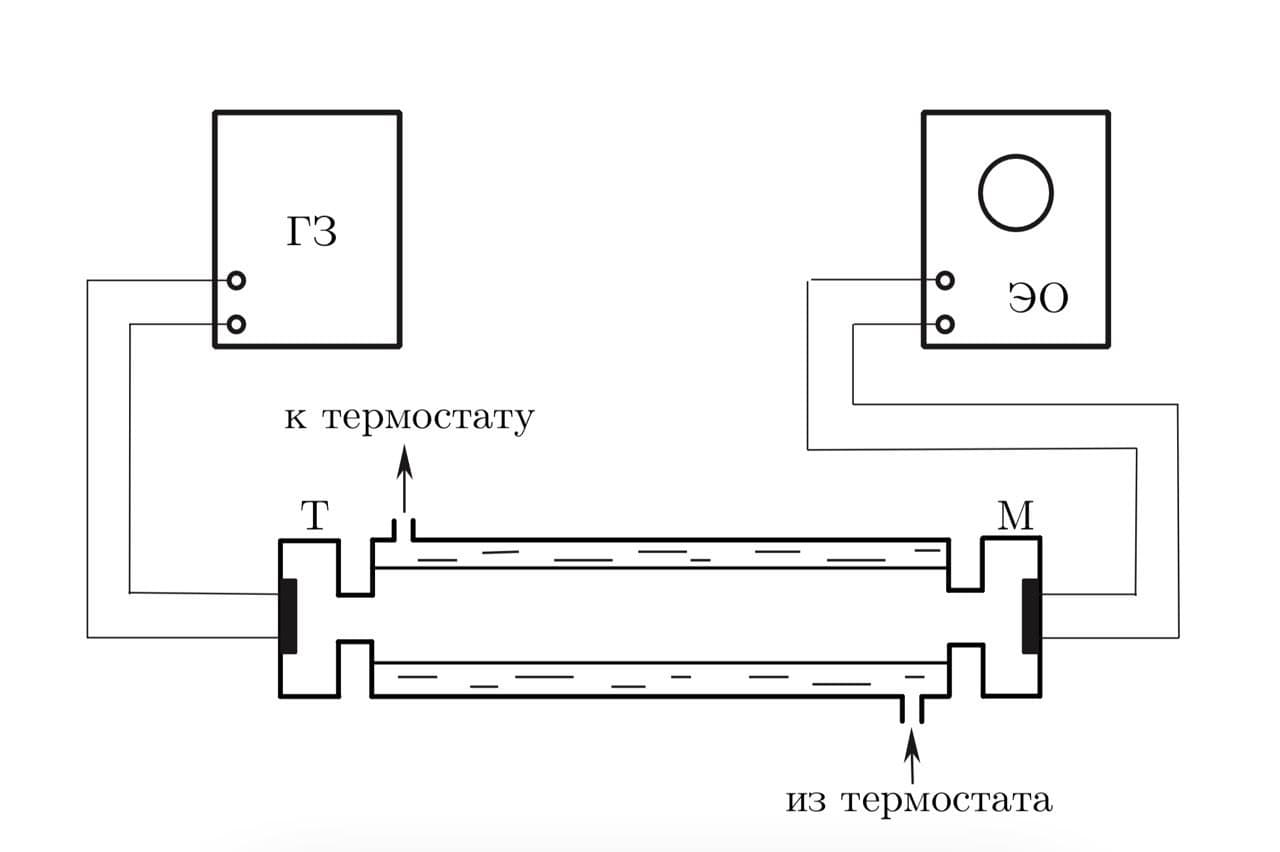
\includegraphics[scale=0.3]{lab213ris1.png}}
\caption{\textit{Схема экспериментальной установки}}
\end{figure}

\subsection*{Ход работы}

Сделаем предварительную оценку диапазона частот, в котором будет идти работа. Из условия резонанса в трубе получим цепочку равенств:

\begin{equation}
c = \lambda_n f_n \, , \, L = n \frac{\lambda_n}{2} \,  \rightarrow \, f_{n}=c \frac{n}{2L}.
\end{equation}

В формуле (2) n – целое число, c – скорость звука, $\lambda_n$ – длина волны n-ного резонанса, $f_n$ – частота n-ного резонанса, L – длина трубы. В ней должно укладываться целое число полуволн. 

Тогда из формул (1) и (2) получаем приблизительное значение, от которого дальше стоит работать:

\[f_1 \approx 217 \, Гц .\]

Будем искать резонансные частоты, при этом увеличивая температуру газа. Результаты измерений выведем в таблице 1 приложения.

\textbf{ } \\

Для каждой каждой температуры найдем значения коэффициентов $k_i = C_i/2L = f_{n_i} / n_i $ из формулы (2). $k_i$ определяется коэффициентом наклоном графика зависимости $f_{n_i}(n_i)$. Построим их по МНК для каждого графика - рисунок 2 приложения.

Из каждого графика мы можем вычислить коэффициент наклона, который из формулы (2) равен $c/2L$. Из формулы (1) видим, что скорость звука зависит от корня из температуры, что оказывается неудобным для получения модели. Для удобства получим линейную зависимость $c^2$ от T - формула (3). 

\begin{equation}
c^2=(\frac{2Lf_n}{n})^2=\frac{\gamma R}{\mu}T = (2Lk_i)^2 \rightarrow (2Lk_i)^2=\frac{\gamma R}{\mu}T.
\end{equation}

Пользуясь формулой (3), мы можем построить зависимость левой части от температуры, из коэффициента пропорциональности которой можем получить искомое значение $C_p/C_v=\gamma$. Значения $k_i$ для каждой температуры получаем из графиков, приведенных на рисунке 2 приложения. Результаты отражены в таблице 2 приложения.

Данные описанной зависимости приведем в таблице 3 приложения, из которой методом наименьших квадратов, получим итоговое значение искомой величины. 

Погрешность, которую даёт МНК, основывается на случайных отклонениях от наилучшего значения коэффициента. Она не учитывает погрешность приборов, что оказывается критичным ввиду плохо работающего генератора. Его погрешность можно оценить в 5 Гц. Учтем это проведением аналогичных вычислений для граничных частот: к имеющимся резонансным частотам прибавим и вычтем 5 Герц. Из исходных данных получаем следующее коэффициента наклона, из которого вычисляем искомый показатель адиабаты:

\begin{equation}
\gamma = (143 \pm 2) \cdot 10^{-2}.
\end{equation}

\subsection*{Обсуждение результатов}

Экспериментально было получено (4) значение показателя адиабаты воздуха. Справочники диктуют следующее число: 1,4. Как видно, оно близко к полученному. Небольшое расхождение обсуловлено неточностью определения резонансых частот. Во-первых, регистрация резонанса происходит глазом экспериментатора, что уже является довольно грубым способом. Во-вторых, имеет место весомая погрешность звукового генератора. Но все же вкупе эти факторы отклоняют результат от истинного на $1-2\%$. 

\subsection*{Использованная литература}

1.Лабораторный практикум по общей физике: учебное пособие. В трёх томах. Т.1. Термодинамика и молекулярная физика. 3-е изд., испр. / Гладун А.Д., Александров Д.А., Игошин Ф.Ф. и др.; Под ред. А.Д.Гладуна. – М.:МФТИ,2012 – 292с.

\newpage

\subsection*{Приложение}

\begin{table}[htb]
\centering
\caption{\textit{Частоты (в Гц) последовательных резонансов при разных температурах}}
\begin{tabular}{|c|c|c|c|c|c|c|c|c|c|}
\hline
\textbf{n $\backslash$ T [К]} & \textbf{293} & \textbf{298} & \textbf{303} & \textbf{308} & \textbf{313} & \textbf{318} & \textbf{323} & \textbf{328} & \textbf{333} \\ \hline
\textbf{1}                    & 226          & 201          & 205          & 211          & 212          & 215          & 221          & 221          & 225          \\ \hline
\textbf{2}                    & 445          & 448          & 456          & 457          & 459          & 464          & 466          & 469          & 475          \\ \hline
\textbf{3}                    & 655          & 659          & 665          & 659          & 674          & 680          & 693          & 696          & 701          \\ \hline
\textbf{4}                    & 869          & 874          & 881          & 884          & 892          & 902          & 908          & 917          & 921          \\ \hline
\textbf{5}                    & 1080         & 1091         & 1099         & 1101         & 1114         & 1126         & 1128         & 1132         & 1139         \\ \hline
\end{tabular}
\end{table}

\begin{table}[ht]
\centering
\caption{\textit{Коэффициенты $k_i$, вычисленные МНК для каждой температуры}}
\scalebox{0.85}{
\begin{tabular}{|c|c|c|c|c|c|c|c|c|c|}
\hline
\textbf{$T_i [К]$}          & \textbf{293} & \textbf{298} & \textbf{303} & \textbf{308} & \textbf{313} & \textbf{318} & \textbf{323} & \textbf{328} & \textbf{333} \\ \hline
\textbf{$k_i [Гц]$}          & 217,44       & 218,61       & 220,57       & 220,81       & 223,49       & 225,82       & 227,35       & 228,72       & 230,20       \\ \hline
\textbf{$\sigma_{k_i} [Гц]$} & 0,92         & 1,27         & 1,33         & 1,15         & 1,05         & 1,01         & 1,19         & 1,25         & 1,35         \\ \hline
\textbf{$\varepsilon_{k_i}$} & 0,42\%       & 0,58\%       & 0,60\%       & 0,52\%       & 0,47\%       & 0.45\%       & 0,52\%       & 0,54\%       & 0,59\%       \\ \hline
\end{tabular}
}
\end{table}

\begin{table}[ht]
\centering
\caption{\textit{Вычисление $\gamma$}}
\scalebox{0.73}{
\begin{tabular}{|l|c|c|c|c|c|c|c|c|c|}
\hline
\textbf{${f(T)}_i$}             & 121037,2 & 122342,2 & 124543,8 & 124821,1 & 127863,2 & 130546,4 & 132326,6 & 133925,1 & 135659,6 \\ \hline
\textbf{$\varepsilon_{f(T)_i}$} & 0,85\%   & 1,16\%   & 1,20\%   & 1,04\%   & 0,94\%   & 0,89\%   & 1,05\%   & 1,09\%   & 1,17\%   \\ \hline
\textbf{$\sigma_{f(T)_i}$}      & 1025,3   & 1420,3   & 1500,3   & 1303,7   & 1200,4   & 1166,8   & 1386,1   & 1458,1   & 1591,1   \\ \hline
\textbf{$T_i$}                  & 293      & 298      & 303      & 308      & 313      & 318      & 323      & 328      & 333      \\ \hline
\end{tabular}
}
\end{table}

\begin{figure}[]
\center{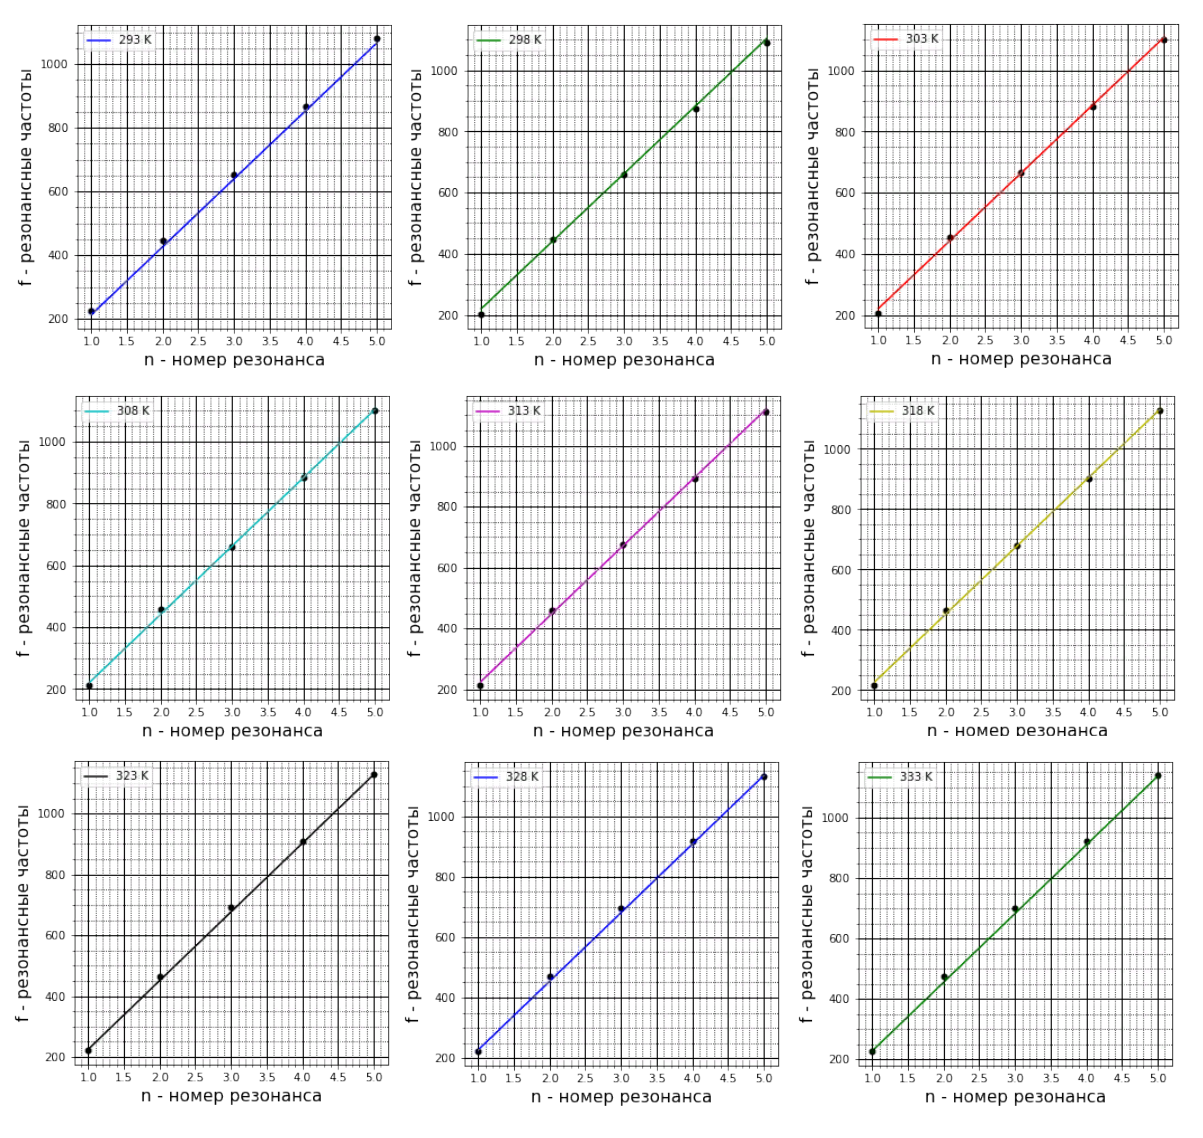
\includegraphics[scale=0.65]{lab213ris2.png}}
\caption{\textit{Графики зависимости резонансной частоты от порядка резонанса при разных температурах}}
\end{figure}

\begin{figure}[]
\center{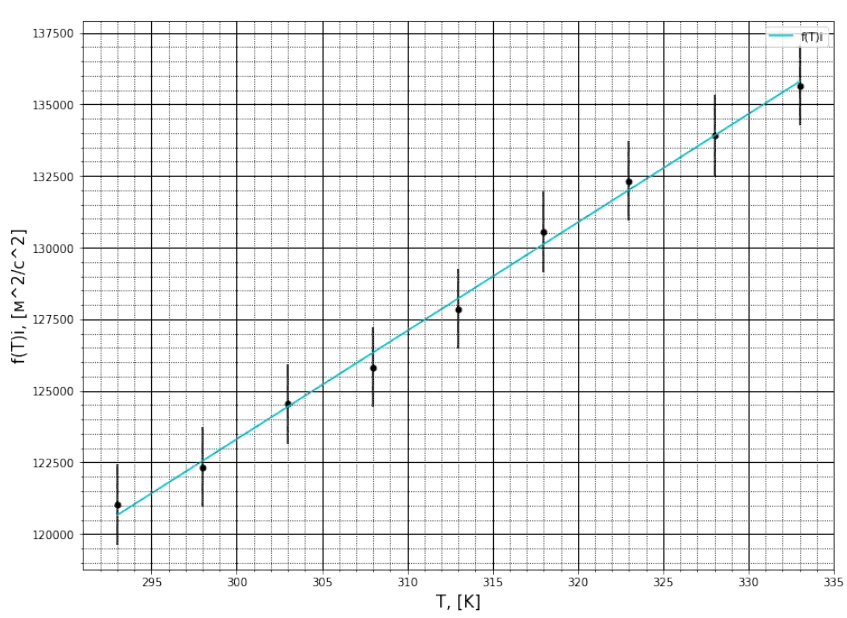
\includegraphics[scale=0.9]{lab213ris3.png}}
\caption{\textit{График зависимости квадрата скорости звука от температуры, коэффициент наклона которой определяет показатель адиабаты}}
\end{figure}

\end{document}
 